A trend we have been seeing lately in the DoD is the misuse of the Assess Only framework. The Assess Only process was created to provide a way of assessing unique technologies below the system level which do not require an authorization like an Authority to Operate, Authority to Connect, Authority to Test, or their interim kin (ATO, ATC, ATT, IATO, IATC, IATT).\autocite[\pno~13]{20240212:dodi851001}

Misusing the Assess Only process results in a security hole. The primary result of misuse includes bypassing the Assess \& Authorize (A\&A) process protections. This evasion of the A\&A process results in increased operational risk, inadequate risk management, a lack of accountability, and a misalignment with mission requirements. To help organizations identify their holes in Assess Only processes, the following items provide a litmus test for making sure that your organization does not abuse RMF policies in a dangerous way:

\subsection{Assess Only Systems}
Referring to ``Assess Only Systems'' indicates a lack of understanding of what may go through the Assess Only process. Systems (including Major Applications, PIT Systems, and SIS/CRNs) must go through the Assess \& Authorize process. Organizations that refer to ``Assess Only Systems'' demonstrate a misunderstanding of what an assessment approval is intended to accomplish. Words have meaning, and using the wrong words creates an inconsistency which introduces weaknesses in a cybersecurity program.

The guidance in DoDI 8500.01 (Figure~\ref{fig:20240212:dodit}) can help in understanding this distinction.\autocite{20240212:dodi850001} Systems do not qualify for the Assess Only process.

\begin{figure}[h]
\centering
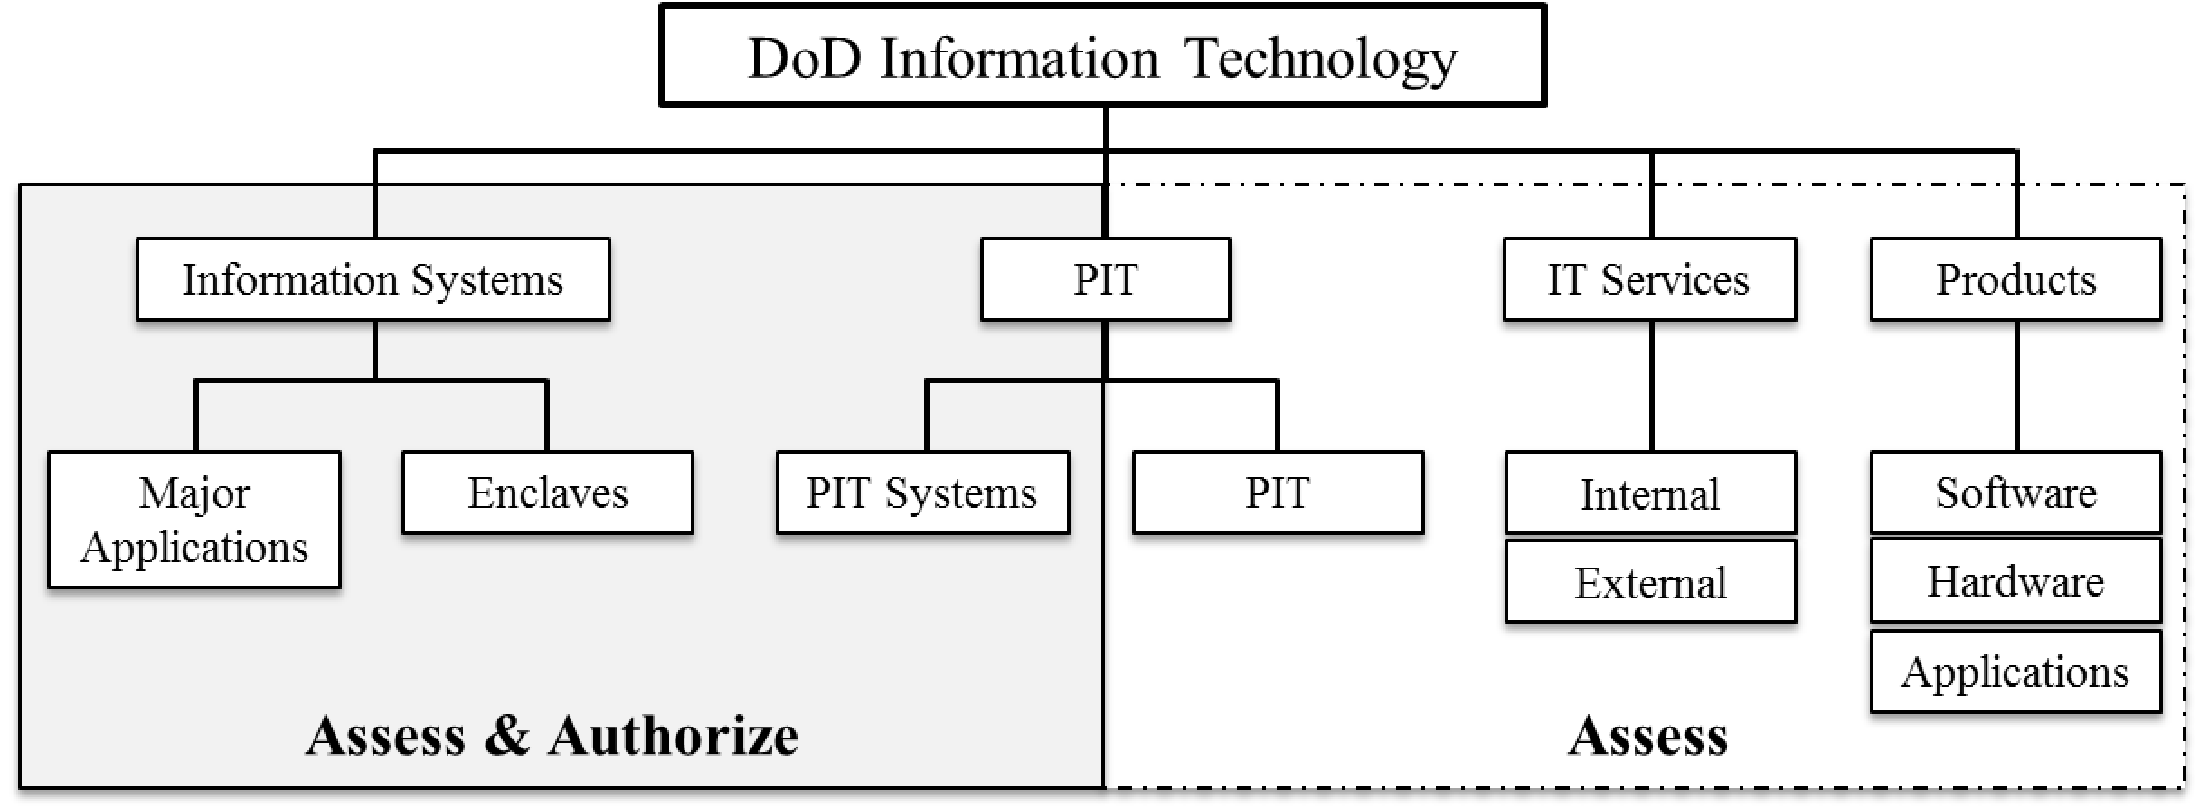
\includegraphics[width=14cm, height=5.144cm]{20240212.dodit.png}
\caption{Assess Only and Assess \& Authorize in DoD Policy}
\label{fig:20240212:dodit}
\end{figure}

\subsection{What is Being Approved}
There are two flavors of the Assess Only process. A program may use the \textit{Assess \& Approve} process to approve single-purpose, non-connecting IT-enabled devices and services, or they can use the \textit{Assess \& Incorporate} process to approve an assessment which can be associated with or incorporated into an already authorized boundary.\autocite[\pno~11]{20240212:vaglia2017} For software applications, notice that the assessment is the focal point of the approval, and the system that wants to associate with that assessment should have a process for incorporating it into their boundary.

Reciprocity requires the incorporating organization to perform due diligence when associating with an approved assessment, and that includes review of the assessment data. Organizations that treat an Assessment Approval of software as if it were a blanket, protean approval of the product (rather than an approval of the assessment) are bypassing the authorization mechanism in RMF and the reciprocity controls of their organization if the process does not include reviewing the assessment data.

\subsection{Assess Only ATO, ATC, and ATT}
An ATO, ATC, and ATT (and by extension, their interim cousins, IATO, IATC, and IATT) begin with the word \textit{Authority}. An \textit{Authorization} requires the Assess \textit{\& Authorize} process. By definition, an Assess Only is not used in the place of an operational authorization.

An authorized boundary which does have an ATO, ATC, or ATT may define policies for associating with an approved assessment to become an authority for the operation of IT below the system level. Those policies should include the review of Assess Only data; however, systems and networks, like the DODIN, may require a full ATO or ATC under the A\&A process.\autocite{20240212:disncpg}

Organizations which refer to an ``Assess Only ATO'' or ``Assess Only ATC'' are trying to mix Step 6 of the RMF process (Authorization) with an approval mechanism that ends at Step 5 (Assessment).

\subsection{Assess Only ConMon}
Taking the misuse of the Assess Only construct a step further are organizations which refer to an ``Assess Only ConMon.'' These organizations attempt to implement Step 7 of the RMF process (Monitoring) in non-standard ways. \textit{Monitoring} in the RMF process refers to the surveillance of authorized assets and controls approved in the Step 6 (Authorized) boundary.\autocite{20240212:nist80037rev2} This is one of the reasons why DoD elements often refer to this as a ConMon Authorization or Continuous ATO (cATO). Consider the wheel in Figure~\ref{fig:20240212:rmfwheel} to help understand where authorization and monitoring fall in the RMF process.

\begin{figure}[h]
\centering
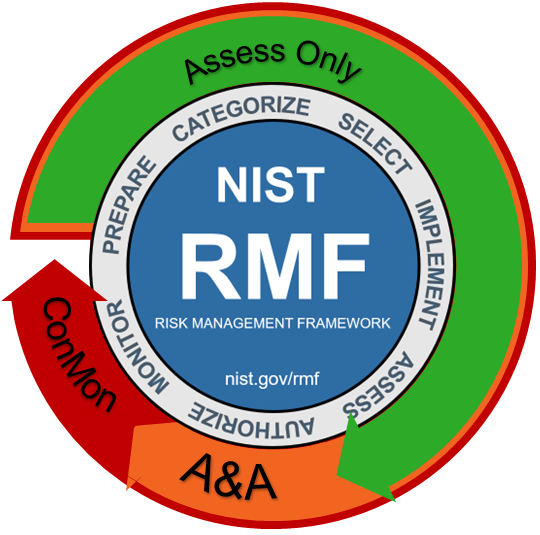
\includegraphics[width=10cm, height=9.73cm]{20240212.rmfwheel.png}
\caption{RMF Process Wheel}
\label{fig:20240212:rmfwheel}
\end{figure}

Continuous monitoring (ConMon) is a requirement for a robust continuous authorization process. It is an \textit{operational} construct which is why it requires an Authority to \textit{Operate} (ATO). Organizations can implement continuous assessment for products below the system level, but to redefine continuous monitoring as meaning continuous assessment gives organizations a false sense of security by bypassing Authorization and answering the final RMF step at the wrong level.

\subsection{Conclusion}
Organizations trying to implement the RMF process should be commended. A program doing their due diligence to implement cybersecurity principles should consider the litmus test provided here to determine if their processes comply with existing DoD guidance.
